% ============================================================
% So sánh Backbone: CNN vs Transformer (YOLOv8s vs DETR)
% Subsection bổ sung vào Section "Kiến trúc Mô hình Học Sâu"
% ============================================================

\subsection{3. Phương pháp DETR (Kiến trúc Transformer-based / Set Prediction)}

Ngoài hai trường phái kinh điển One-stage (YOLOv8) và Two-stage (Faster R-CNN) thuần CNN đã phân tích ở trên, nhóm mở rộng nghiên cứu sang hướng tiếp cận thứ ba mang tính cách mạng: \textbf{DETR (DEtection TRansformer)} --- mô hình đầu tiên áp dụng kiến trúc Transformer vào bài toán Object Detection, được giới thiệu bởi Carion et al. tại Facebook AI Research (ECCV 2020). DETR tái định nghĩa hoàn toàn bài toán phát hiện đối tượng từ mô hình hồi quy hộp truyền thống sang bài toán \textbf{dự đoán tập hợp (Set Prediction)}, loại bỏ triệt để các thành phần thủ công như anchor boxes, NMS, và region proposals.

Mục đích của việc bổ sung DETR nhằm đáp ứng yêu cầu đề bài mục 4.2: \textit{``Backbone hoặc kiến trúc khác nhau (CNN vs Transformer)''} --- so sánh trực tiếp phương pháp trích xuất đặc trưng thuần CNN (YOLOv8 với CSPDarknet) và phương pháp kết hợp CNN + Transformer (DETR với ResNet-50 + Transformer Encoder-Decoder).

\begin{lstlisting}[language=Python, caption=Khởi tạo và cấu hình Transfer Learning DETR]
from transformers import DetrForObjectDetection

detr_model = DetrForObjectDetection.from_pretrained(
    'facebook/detr-resnet-50',
    num_labels=NUM_CLASSES,       # 7 lop KITTI
    ignore_mismatched_sizes=True  # thay doi classification head
).to(device)
\end{lstlisting}

\subsubsection*{Phân tích Chuyên sâu Cấu trúc DETR}

\begin{figure}[H]
	\centering
	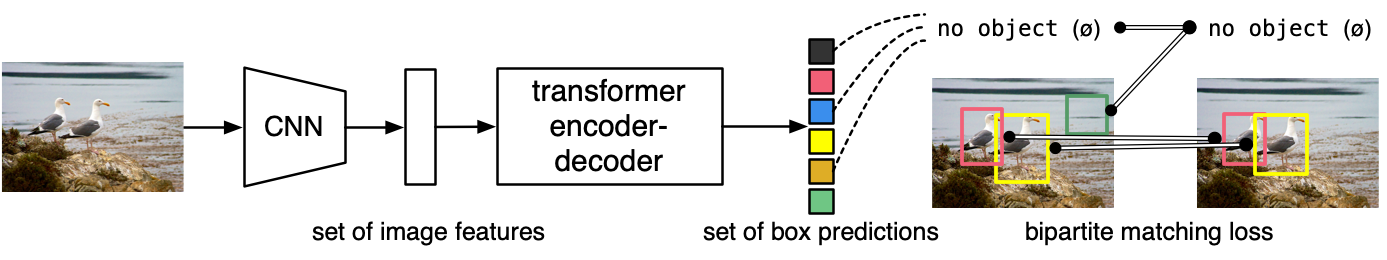
\includegraphics[width=\textwidth]{Images/detr-architecture.png}
	\caption{Kiến trúc tổng quan DETR: Backbone CNN (ResNet-50) trích xuất feature map, Transformer Encoder mã hóa ngữ cảnh toàn cục qua self-attention, Transformer Decoder nhận $N$ object queries và sinh ra dự đoán song song, cuối cùng FFN heads xuất lớp và tọa độ bounding box. Nguồn: Carion et al., ECCV 2020.}
	\label{fig:detr-arch}
\end{figure}

\begin{itemize}
	\item \textbf{Tầng Trích xuất Đặc trưng (Backbone --- ResNet-50):} Khác với YOLOv8 sử dụng CSPDarknet tự thiết kế, DETR tái sử dụng mạng ResNet-50 truyền thống làm backbone CNN để trích xuất feature map từ ảnh đầu vào. Ảnh gốc có kích thước $H_0 \times W_0 \times 3$ được đưa qua ResNet-50, tạo ra feature map kích thước $\frac{H_0}{32} \times \frac{W_0}{32} \times 2048$. Tiếp đó, một lớp tích chập $1 \times 1$ chiếu giảm chiều từ 2048 kênh xuống còn $d = 256$ kênh, tạo thành tensor đặc trưng $\frac{H_0}{32} \times \frac{W_0}{32} \times 256$. Điểm mấu chốt ở đây: \textbf{backbone ResNet-50 chỉ trích xuất đặc trưng cục bộ (local features) thông qua phép tích chập, hoàn toàn không có khả năng nắm bắt quan hệ toàn cục} --- nhiệm vụ này được ủy thác cho Transformer Encoder ở tầng tiếp theo.

	\item \textbf{Mã hóa Vị trí Không gian (Positional Encoding):} Do cơ chế self-attention trong Transformer bản chất là \textit{permutation-invariant} (không phân biệt thứ tự), DETR bổ sung \textbf{Fixed Sinusoidal Positional Encoding} trực tiếp cộng vào feature map đã flatten. Mỗi vị trí $(x, y)$ trên feature map được mã hóa bằng cặp hàm $\sin$ và $\cos$ ở nhiều tần số khác nhau theo cả hai chiều không gian:
	$$PE_{(pos, 2i)} = \sin\left(\frac{pos}{10000^{2i/d}}\right), \quad PE_{(pos, 2i+1)} = \cos\left(\frac{pos}{10000^{2i/d}}\right)$$
	Kỹ thuật này cho phép Transformer phân biệt chính xác vị trí không gian của từng pixel đặc trưng, bù đắp khuyết thiếu mà pure attention không thể tự học. So sánh với YOLOv8: YOLO giữ nguyên cấu trúc không gian qua Grid Cell nên không cần encoding riêng; DETR flatten toàn bộ feature map thành sequence 1D nên bắt buộc cần bước này.

	\item \textbf{Bộ Mã hóa Transformer (Transformer Encoder --- Global Context):} Feature map sau khi flatten thành sequence gồm $\frac{H_0}{32} \times \frac{W_0}{32}$ token được nạp vào stack gồm \textbf{6 lớp Transformer Encoder}. Mỗi lớp encoder thực hiện:
	\begin{enumerate}
		\item \textbf{Multi-Head Self-Attention:} Mỗi vị trí trên feature map ``nhìn thấy'' \textit{tất cả} các vị trí khác thông qua cơ chế attention trọng số mềm. Đây là bước đột phá so với CNN truyền thống (chỉ nhìn receptive field cục bộ). Với KITTI --- nơi đoàn xe xếp hàng dài tại ngã tư, một chiếc xe ở góc trái ảnh có thể tham chiếu đến ngữ cảnh giao thông ở góc phải, giúp DETR phân biệt từng xe riêng biệt ngay cả khi chúng chồng lấn.
		\item \textbf{Feed-Forward Network (FFN):} Mạng 2 lớp fully-connected với hàm kích hoạt ReLU xử lý phi tuyến từng vị trí độc lập.
		\item \textbf{Layer Normalization + Residual Connection:} Ổn định gradient và tăng tốc hội tụ.
	\end{enumerate}
	Tuy nhiên, cơ chế self-attention có \textbf{độ phức tạp $O(n^2)$} với $n = H/32 \times W/32$ --- đây là nguyên nhân cốt lõi khiến DETR tiêu tốn GPU memory gấp bội so với YOLOv8 và giới hạn batch size xuống còn 4 (so với 16 của YOLOv8).

	\item \textbf{Bộ Giải mã Transformer (Transformer Decoder --- Object Queries):} Thành phần cách mạng nhất của DETR nằm ở \textbf{Transformer Decoder} với $N = 100$ \textbf{object queries} --- đây là $N$ learned embeddings được khởi tạo ngẫu nhiên và học qua quá trình training. Mỗi object query đóng vai trò như một ``đầu dò'' chuyên trách phát hiện tối đa một đối tượng. Stack gồm \textbf{6 lớp Transformer Decoder}, mỗi lớp thực hiện:
	\begin{enumerate}
		\item \textbf{Self-Attention giữa các object queries:} Cho phép các ``đầu dò'' giao tiếp với nhau, tránh hai query cùng bắt một đối tượng (giải quyết bài toán duplicate detection mà NMS truyền thống phải xử lý hậu kỳ).
		\item \textbf{Cross-Attention với encoder output:} Mỗi object query truy vấn vào toàn bộ feature map đã được encoder mã hóa ngữ cảnh, tập trung chú ý (attend) vào khu vực ảnh chứa đối tượng mà nó ``chịu trách nhiệm''.
	\end{enumerate}
	Cơ chế này thay thế hoàn toàn bước Region Proposal + NMS của Faster R-CNN và bước Grid Cell + NMS của YOLOv8. Kết quả: \textbf{DETR xuất trực tiếp tập hợp $N$ dự đoán song song}, không cần bất kỳ hậu xử lý nào.

	\item \textbf{Đầu Dự đoán (Prediction FFN Heads):} Mỗi object query sau decoder được đưa qua hai nhánh FFN song song:
	\begin{itemize}
		\item \textbf{Classification Head:} Softmax phân loại $C + 1$ lớp (bao gồm lớp đặc biệt $\varnothing$ = ``no object'' cho các query không bắt được đối tượng nào).
		\item \textbf{Box Regression Head:} FFN 3 lớp với hàm kích hoạt sigmoid, dự đoán 4 giá trị normalized: $(c_x, c_y, w, h)$ --- tọa độ tâm và kích thước bounding box.
	\end{itemize}

	\item \textbf{Hàm Mất mát Hungarian Matching (Bipartite Matching Loss):} Đây là nền tảng lý thuyết cốt lõi phân biệt DETR với mọi detector trước đó. Thay vì dùng IoU threshold cứng để gán label (như Faster R-CNN, YOLOv8), DETR sử dụng \textbf{thuật toán Hungarian} để tìm phép gán tối ưu 1-1 giữa $N$ predictions và $M$ ground-truth objects (với $M \ll N$, các prediction thừa được gán lớp $\varnothing$). Hàm cost kết hợp:
	$$\mathcal{L}_{Hungarian} = \lambda_{cls} \cdot \mathcal{L}_{cls} + \lambda_{L1} \cdot \mathcal{L}_{L1} + \lambda_{giou} \cdot \mathcal{L}_{GIoU}$$
	Trong đó $\mathcal{L}_{cls}$ là cross-entropy cho phân loại, $\mathcal{L}_{L1}$ là L1 loss cho tọa độ box, và $\mathcal{L}_{GIoU}$ là Generalized IoU loss cho hình dạng box. Ưu điểm: đảm bảo mỗi đối tượng \textit{chỉ được dự đoán đúng một lần}, loại bỏ hoàn toàn nhu cầu NMS. Nhược điểm: quá trình matching phức tạp khiến \textbf{DETR hội tụ rất chậm} --- paper gốc cần 300 epochs trên COCO, trong khi YOLOv8 chỉ cần 50--100 epochs.
\end{itemize}

\subsection{4. So sánh đặc điểm kiến trúc: CNN-based (YOLOv8) vs Transformer-based (DETR)}

Để đáp ứng yêu cầu đề bài mục 4.2 --- \textit{``Backbone hoặc kiến trúc khác nhau (CNN vs Transformer)''}, Bảng~\ref{tab:cnn-vs-transformer} tổng hợp đối chiếu giữa phương pháp thuần CNN (YOLOv8s) và phương pháp kết hợp Transformer (DETR) trên cùng tập dữ liệu KITTI:

\begin{table}[H]
\centering
\caption{Đối chiếu kiến trúc CNN-based (YOLOv8s) vs Transformer-based (DETR) trên KITTI.}
\label{tab:cnn-vs-transformer}
\begin{tabular}{|l|p{5.2cm}|p{5.2cm}|}
\hline
\textbf{Tiêu chí} & \textbf{YOLOv8s (CNN-based)} & \textbf{DETR (Transformer-based)} \\
\hline
Backbone & CSPDarknet (thuần CNN) & ResNet-50 (CNN) + Transformer Encoder-Decoder \\
\hline
Cơ chế trích xuất đặc trưng & Tích chập cục bộ (local convolutions) qua nhiều tầng, kết hợp FPN đa tỉ lệ & Tích chập cục bộ (backbone) $\rightarrow$ Self-attention toàn cục (encoder) \\
\hline
Receptive field & Giới hạn bởi kernel size, mở rộng dần qua các tầng sâu & Toàn cục ngay từ tầng encoder đầu tiên ($O(n^2)$ attention) \\
\hline
Cách phát hiện đối tượng & Grid-based, anchor-free, dự đoán trên multi-scale feature maps & Set prediction với $N$ object queries song song, không dùng grid \\
\hline
Hậu xử lý & Cần NMS để loại bỏ box trùng & Không cần NMS --- Hungarian matching đảm bảo 1-1 \\
\hline
Phát hiện đối tượng nhỏ & Tốt nhờ FPN multi-scale (P3, P4, P5) & Hạn chế --- feature map $H/32 \times W/32$ mất chi tiết nhỏ \\
\hline
Phát hiện đối tượng lớn & Tốt & Rất tốt nhờ global attention bao quát toàn ảnh \\
\hline
Tiêu tốn GPU memory & Thấp (batch size 16) & Cao (batch size 4) do $O(n^2)$ self-attention \\
\hline
Tốc độ hội tụ & Nhanh (50 epochs) & Chậm (300 epochs theo paper gốc) \\
\hline
Thiết kế end-to-end & Không hoàn toàn (vẫn cần NMS) & Hoàn toàn end-to-end (không thành phần thủ công) \\
\hline
Pretrained trên & COCO (80 lớp) & COCO (91 lớp) \\
\hline
\end{tabular}
\end{table}

\subsection{5. Cấu hình và Tham số Huấn luyện: YOLOv8s vs DETR}

Bảng~\ref{tab:cnn-transformer-params} tổng hợp toàn bộ tham số huấn luyện của hai mô hình trên cùng tập KITTI:

\begin{table}[H]
\centering
\caption{Đối chiếu tham số huấn luyện YOLOv8s (CNN) và DETR (Transformer) trên KITTI.}
\label{tab:cnn-transformer-params}
\begin{tabular}{|l|c|c|}
\hline
\textbf{Tham số} & \textbf{YOLOv8s} & \textbf{DETR} \\
\hline
Mô hình pretrained & \texttt{yolov8s.pt} (COCO) & \texttt{detr-resnet-50} (COCO) \\
\hline
Kích thước ảnh đầu vào & $640 \times 640$ (resize cố định) & Kích thước gốc (biến đổi) \\
\hline
Batch size & 16 & 4 \\
\hline
Số epochs & 50 & 20 \\
\hline
Optimizer & SGD (momentum = 0.937) & AdamW \\
\hline
Learning rate & 0.01 (toàn bộ mạng) & $10^{-4}$ (head) / $10^{-5}$ (backbone) \\
\hline
LR schedule & Linear decay ($lr_f = 0.01$) & StepLR (step=15, $\gamma$=0.1) \\
\hline
Weight decay & 0.0005 & $10^{-4}$ \\
\hline
Warmup & 3 epochs & --- \\
\hline
Gradient clipping & --- & max\_norm = 0.1 \\
\hline
Seed & 42 & 42 \\
\hline
Số lớp & 7 & 7 \\
\hline
Tập dữ liệu & KITTI (80\% train / 20\% val) & KITTI (80\% train / 20\% val) \\
\hline
\end{tabular}
\end{table}

\textbf{Phân tích sự khác biệt cấu hình:}
\begin{itemize}
	\item \textbf{Batch size (16 vs 4):} DETR tiêu tốn GPU memory lớn hơn đáng kể do cơ chế self-attention $O(n^2)$ trong Transformer encoder. Trên GPU Tesla T4 (16GB VRAM), DETR chỉ cho phép batch size 4, trong khi YOLOv8s thoải mái chạy batch size 16.
	\item \textbf{Optimizer (SGD vs AdamW):} YOLOv8 theo truyền thống YOLO dùng SGD với momentum cao (0.937) và warmup. DETR theo chuẩn Transformer dùng AdamW --- optimizer được thiết kế đặc biệt cho mạng Transformer nhờ cơ chế decoupled weight decay giúp ổn định training attention layers.
	\item \textbf{Learning rate phân tầng:} DETR áp dụng chiến lược differential learning rate: backbone ResNet-50 (đã được pretrained mạnh trên ImageNet) chỉ cần tinh chỉnh nhẹ ($10^{-5}$), trong khi Transformer head cần học nhanh hơn ($10^{-4}$) để thích nghi với phân bố dữ liệu KITTI. YOLOv8 dùng chung một learning rate vì toàn bộ kiến trúc đã được tối ưu đồng bộ từ pretrained COCO.
	\item \textbf{Gradient clipping (chỉ DETR):} Transformer dễ gặp hiện tượng gradient exploding do attention weights nhân ma trận lớn, nên cần clip gradient ở max\_norm = 0.1.
	\item \textbf{Số epochs (50 vs 20):} DETR được train ít epochs hơn (20 thay vì 300 theo paper gốc) do giới hạn thời gian GPU trên Kaggle. Mỗi epoch DETR mất khoảng 3 phút (tổng $\approx 60$ phút), trong khi mỗi epoch YOLOv8 chỉ mất 18 giây (tổng $\approx 15$ phút cho 50 epochs). Điều này phản ánh thực tế về chi phí tính toán Transformer vs CNN.
\end{itemize}
